\documentclass{article}

\usepackage{fullpage}
\usepackage[utf8]{inputenc}
\usepackage{listings}
\usepackage{caption}
\usepackage[table]{xcolor}
\usepackage{amssymb}
\usepackage{amsmath}
\usepackage{fancyhdr}
\usepackage{lastpage}
\usepackage{parskip}
\usepackage{url}
\usepackage{float}
\usepackage{enumitem}
\usepackage{amstext}
\usepackage{fancybox}
\usepackage{amsmath}
\usepackage{stmaryrd}
\usepackage{graphicx}
\usepackage{subcaption}
\usepackage[bottom]{footmisc}
\usepackage{hyperref}

%%% Local Variables:
%%% mode: latex
%%% TeX-master: "index"
%%% End:

\newcommand{\code}[1]{\texttt{#1}}
\newcommand\unfootnote[1]{\let\thefootnote\relax\footnotetext{#1}}
\newcommand{\mc}[1]{\mathcal{#1}}


\pagestyle{fancy}
\fancyhf{}
\setlength{\parindent}{0pt}
\setlength{\headheight}{15pt}
\setlength{\headsep}{25pt}
\lhead{\leftmark}
\cfoot{Page \thepage{} of \pageref{LastPage}}

\title{
  01410 Cryptology 1\\
  Notes
}
\date{May, 2014}
\author{}

\setcounter{section}{-1}

\begin{document}
\maketitle
\clearpage

\tableofcontents
\clearpage

\section{Common}
%%% Local Variables:
%%% mode: latex
%%% TeX-master: "../index"
%%% End:

\subsection{Euclid's Algorithm}
\label{sec:euclids-algorithm}
Finds $\gcd(a, b)$
\begin{align*}
  a = 90,&\quad b = 34 \\
  r_0 &= 90\\
  r_1 &= 34\\
  r_2 &= 90 - 2*34 = 22\\
  r_3 &= 34 - 1*22 = 12\\
  r_4 &= 22 - 1*12 = 10\\
  r_5 &= 12 - 1*10 = 2
\end{align*}
End because 2 divides 10, thus $\gcd(90, 34) = 2$

\subsection{Euclid's Extended Algorithm}
\label{sec:euclids-extended}
\begin{align*}
  s_j = \begin{cases}
    1 &\text{if}\ j = 0\\
    0 &\text{if}\ j = 1\\
    s_{j-2} - q_{j-1}s_{j-1} &\mbox{if} j \ge 2
  \end{cases}\\ \\
  t_j = \begin{cases}
    1 &\text{if}\ j = 0\\
    0 &\text{if}\ j = 1\\
    t_{j-2} - q_{j-1}t_{j-1} &\text{if}\ j \ge 2
  \end{cases}
\end{align*}

\begin{table}[H]
  \centering
  \begin{tabular}{lllll}
    $i$ & $r_i$ & $q_i$ & $s_i$ & $t_i$ \\ \hline
    0   & 90    &       & 1     & 0     \\
    1   & 34    & 2     & 0     & 1     \\
    2   & 22    & 1     & 1     & -2    \\
    3   & 12    & 1     & -1    & 3     \\
    4   & 10    & 1     & 2     & -5    \\
    5   & 2     & 1     & -3    & 8     \\
  \end{tabular}
  \caption{Example run of Euclid's Extended Algorithm}
\end{table}
The output of Euclid's extended algorithm can be written as:
\[ 1 = r \cdot s + t \cdot p\]
Where t will be the multiplicative inverse of $p^{-1} \mod s$.

\subsection{Chinese Remainder Theorem}
\label{sec:crm}
If $x^ay^b \equiv z \mod p$, then $(x^a \mod p)(y^b \mod p) \equiv z \mod p$

Also $x^ay^b \mod p = (x^a \mod p)(y^b \mod p) \mod p$

\subsection{Modular Multiplicative Inverse}
\label{sec:modular-mult-inverse}
Modular multiplicative inverse of $a \mod m$ is $x$ in
\[ ax \equiv 1 \mod m \]
where $x = a^{-1} \mod m$.

$a$ must be ``coprime'' to $m$ ($\gcd(a, m) = 1$).

\textbf{Ex} $3^{-1} \mod m = 4$, because $3 \cdot 4 = 12 \equiv 1 \mod 4$

Can be found using Euclid's Extended Algorithm~(\ref{sec:euclids-extended}).
\[ 1 = r \cdot s + t \cdot p\]
where t is the multiplicative inverse.
\subsection{Euler's $\phi$-function}
\label{sec:eulers-phi}
Defines the number of $a \in \mathbb{Z}_p$ for which $\gcd(a, p) = 1$,
e.i. number of coprimes to $p$ in $\mathbb{Z}_p$.

\subsection{Fermat's Little Theorem}
\label{sec:fermats-little}
For all $b \in \mathbb{Z}_p^*$ it holds that $b^{p-1} \equiv 1 \mod
p$, where $p$ is a prime.

\subsubsection*{Proof}
Given the set
\[ \mathbb{Z}_p^* = \{1,2,3,\ldots,p-1\} \]

we can multiply some element $b \in \mathbb{Z}_p^*$ onto all elements,
and get the set
\[ \{b,2b,\ldots,b(p-1)\} \mod p \]
since we know that none of the elements is congruent to zero modulo
$p$ from Theorem 2.4.3 we know $ab \equiv 0 \mod p$ if $a \lor b \equiv 0 \mod
p$.

From that it is also known that both sets are equal. Since
multiplication is commutative, we get:
\begin{align*}
  1 \cdot 2 \cdot \ldots \cdot (p - 1) \mod p &= b \cdot 2b \cdot \ldots
  \cdot b(p-1) \mod p\\
  &= b^{p-1}(1\cdot 2 \cdot \ldots \cdot (p - 1)) \mod p
\end{align*}

From the before mentioned theorem, it is also known that the left-hand
side has a multiplicative inverse due to $1 \cdot 2 \cdot \ldots \cdot
(p - 1) \not \equiv 0 \mod p$. If that is multiplied on each side we
get Fermat's Little Theorem:
\[b^{p-1} \equiv 1 \mod p \]

\subsection{Theorem 2.4.3}
Let $p$ be a prime and let $a,b \in \mathbb{Z}$ Then it holds that
\[ ab \equiv 0 \mod p \Rightarrow a \equiv 0 \mod p \; \lor \; b
\equiv 0 \mod p\]

\subsubsection*{Proof}
Assume $ab \equiv 0 \mod p$.

If $a \equiv 0 \mod p$ we are done. So we need to show nif $a \not
\equiv 0 \mod p$ then $b \equiv 0 \mod p$.

Since $a \not \equiv 0$ for $a \in \mathbb{Z}_p^*$, it has a
multiplicative inverse modulo $p$
\[ ac \equiv 1 \mod p \]

Thus we can see
\[ b = 1 \cdot b = (ca)b=c(ab) = c \cdot 0 = 0 \]
\clearpage

\section{Symmetric encryption and public-key encryption}
%%% Local Variables: 
%%% mode: latex
%%% TeX-master: "../index"
%%% End: 

% Recommended:
% Show symmetric-key example with Alice-Bob diagram
% Mention modern algorithm (e.g. AES, Triple-DES)
% Benefits of public-key encryption (no key sharing)
% Show public-key example with RSA and Alice-Bob diagram
\subsection{Agenda}
\begin{enumerate}
\item Symmetric-key encryption
\item Symmetric- vs. public-key encryption
\item RSA
\end{enumerate}
\subsection{Symmetric-key encryption}
\subsubsection{Set up}
\begin{itemize}
  \item $m \in \mathcal{P}$ is the plaintext
  \item $k \in \mathcal{K}$ is the key
  \item $c \in \mathcal{C}$ is the ciphertext
  \item $e_k(m)$ encryption function
  \item $d_k(c)$ decryption function
\end{itemize}

\begin{figure}[H]
  \begin{centering}
    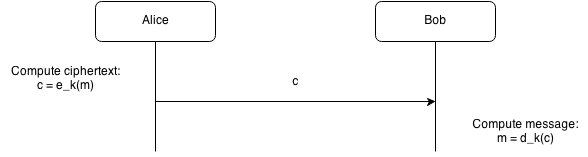
\includegraphics[width=15cm]{images/1-sym-enc}
    \caption{Basic model for symmetric encryption}
  \end{centering}
  \label{fig:sym-enc}
\end{figure}

\subsubsection{Modern implementations}
\begin{description}
\item[DES] 64-bit block cipher with 56-bit key. Due to small key,
  exhaustive search is a possibility. Therefore, \emph{Triple-DES} was
  made.
\item[AES] 128-bit block cipher with 128 to 256-bit key.
\end{description}

\subsection{Symmetric- vs. public-key encryption}
\begin{description}
\item[Pros] Faster and easier to implement
\item[Cons] Requires both parties can access the secret key. Impossible?
\end{description}

\subsection*{RSA}
\begin{itemize}
\item Public key = (n,e) 
\item Private key = (p,q,d) where $ed \equiv 1 mod \phi (n)$.
\item Encryption is done by $Enc(m)= m^e mod n$.
\item Decryption is done by $Dec(c)=c^d mod n$.	
\item n = 2 primes p and q (pq=n)(big primes makes encryption safer)
\item e = is an integer $\in \mathbb{Z}^*_{\phi (n)}$, where $\phi (n)=(p-1)(q-1)$
\item d = is the multiplicative inverse of $e\; mod\;\phi (n)$
\end{itemize}
\subsubsection{Weakness}
\begin{itemize}
\item Attacker can get factors of n
\begin{itemize}
\item if attacker can factor n then he can find d same way that the system computes it
\end{itemize}
\item Attacker finds $\phi (n)$, then factors n
\begin{itemize}
\item if n is small attacker can setup an equation with two unknowns that uses $\phi (n)=(p-1)(q-1)$ since he knows $n=pq$
\begin{align*}
\phi (n)=n-p-q+1=>p&=n-\phi (n)-q+1\\
\mbox{since } p&=\frac{n}{q}\\
\frac{n}{q}&=n-\phi (n)-q+1\\
0&=q^2+q(\phi (n)-n-1)+n
\end{align*}
\end{itemize}
\item Attacker finds the decryption exponent d, then factors n
\begin{itemize}
\item If the attacker finds d its easy to factor n.
\end{itemize}
\item If $c_1$ and $c_2$ are encrypted with the same key then:
\begin{align*}
&(c_1c_2)^d\; mod\; n = (c_1^d) (c_2^d)\; mod \;n\\
&\mbox{which means}\\
&(c_1^d) (c_2^d)\; mod \;n = m_1m_2\;mod \; n
\end{align*}



\end{itemize}
\subsubsection{Example}
Alice and bob each have their individual private and public keys.
If alice wants to send an encrypted message to bob she needs his public key which she gets automatically.\\
Alice now encrypts her message $Enc(m)=m^e_{Bob}\;mod\;n_{Bob}$ and sends it to Bob. \\
Bob now has the ciphertext which needs to be decrypted. Since the message was encrypted with his public key his private key can decrypt it. $Dec(c_{Alice})=\;c^{d_{Bob}}_{Alice}\;mod\;n_{Bob}$.\\
Bob now gets Alice’s message.

\subsubsection{Proof}
%%% Local Variables:
%%% mode: latex
%%% TeX-master: "../index"
%%% End:

\textbf{Public:} $n = pq$ for primes $p, q$ and encryption exponent $e
\in \mathbb{Z}_{\phi(n)}^*$

\textbf{Private:} $(p, q, d)$ where $d \in \mathbb{Z}_{\phi(n)}^*$, such that
\[ ed \equiv 1 \mod \phi(n) \]

Define $\phi(n) = (p-1)(q-1)$. We have that
\begin{align*}
  & ed \equiv 1 \mod \phi(n)\\
  \Rightarrow\quad& ed = 1 + k(p - 1)(q - 1) \quad \text{where } k \in \mathbb{Z}
\end{align*}

We need to prove that $(m^e)^d \equiv m \mod$ since that is enc and dec using RSA.
\begin{align*}
(m^e)^d &\equiv m \mod n \\
\Rightarrow\quad m^{ed} &\equiv m \mod n
\end{align*}

Chinese remainder says that it is enough to show
\[ m^{ed} \equiv m \mod p \textbf{ and } m^{ed} \equiv m \mod q \]

Showing for $p$. There are two cases: 1) $m \equiv 0 \mod p$ and 2) $m \not\equiv 0 \mod p$.

\textbf{Case 1}
\begin{align*}
m &\equiv 0 \mod p\\
\Rightarrow\quad m^x &\equiv m \mod p \quad \text{where } x \in \mathbb{Z}
\end{align*}
and since $ed \in \mathbb{Z}$ case 1 holds.

\textbf{Case 2}
\begin{align*}
m^{ed} &\equiv m \mod p\\
m^{1 + k(p-1)(q-1)} &\equiv m \mod p\\
m \cdot m^{k(p-1)(q-1)} &\equiv m \mod p\\
m \cdot (m^{(p-1)})^{k(q-1)} &\equiv m \mod p
\end{align*}

From \textbf{Fermats little theorem} (\ref{sec:fermats-little}) we
know that $x^{p-1} \equiv x \mod p$ for prime $p$. Thus
\begin{align*}
m \cdot 1^{k(q-1)} &\equiv m \mod p\\
m \cdot 1 &\equiv m \mod p\\
m &\equiv m \mod p
\end{align*}

Therefore, case 2 also holds and we have proved for prime $p$.


\clearpage

\section{Symmetric-key authentication and public-key authentication}
%%% Local Variables:
%%% mode: latex
%%% TeX-master: "../index"
%%% End:

\subsection{Recommended}
\begin{itemize}
\item Show example (e.g. RSA)
\item Alice-Bob diagram
\end{itemize}

\clearpage

\section{Vigenere encryption and cryptanalysis}
%%% Local Variables:
%%% mode: latex
%%% TeX-master: "../index"
%%% End:

\subsection{Recommended}
\begin{itemize}
\item Explain Vigenere
\item Must include cryptoanalysis
  \begin{itemize}
  \item Remember formulas
  \item Index of coincidence
  \end{itemize}
\end{itemize}

\clearpage

\section{Block ciphers, modes of operation, CBC-MAC}
%%% Local Variables:
%%% mode: latex
%%% TeX-master: "../index"
%%% End:

% Recommended:
% Explain with AES (not an requirement)
% Why do we chain blocks?
% Do example with matrix
% CBC-MAC

\subsection*{Agenda}
\begin{enumerate}
\item Block ciphers
\item AES
\item Modes of operation
\item CBC-MAC
\end{enumerate}

\clearpage

\section{RSA public-key encryption}
%%% Local Variables:
%%% mode: latex
%%% TeX-master: "../index"
%%% End:

% Recommended:
% Why does it work?!
% Prime generation
% Modulus exponentiation
% Alice-Bob diagram

\subsection*{Agenda}
\begin{enumerate}
\item Setup
\item Prime generation
\item Modulus exponentiation
\item Proof
\end{enumerate}

\subsection{Setup}
\textbf{Public key:} $(n, e)$ where $n = pq$ for primes $p, q$ and $e \in \mathbb{Z}_{\phi(n)}^*$

\textbf{Private key:} $(p, q, d)$ where $d \in \mathbb{Z}_{\phi(n)}^*$, such that
\[ ed \equiv 1 \mod \phi(n) \]

We use $\phi(n)$ because it is hard to compute given only a large $n$, but easy with known $p, q$ since $\phi(n) = (p-1)(q-1)$, thus $d$ cannot be easily computed given just $n$ (must prime factor $n$).

\textbf{Encryption:} $m$ is the message. Encryption is
\[ Enc(m) = m^e \mod n \]

\textbf{Decryption:} $c$ is the ciphertext. Decryption is as follows:
\[ Dec(c) \equiv c^d \mod n \]
\[ Dec(c) \equiv m^{ed} \mod n \]

\textbf{Properties of RSA:}

$e$ must be chosen such that it holds that $gcd(\phi(n),e) = 1$, where
$\phi(n) = (p - 1)(q - 1)$

$n$ must be the product of two large primes $p$ and $q$.

\subsection{Proof}
%%% Local Variables:
%%% mode: latex
%%% TeX-master: "../index"
%%% End:

\textbf{Public:} $n = pq$ for primes $p, q$ and encryption exponent $e
\in \mathbb{Z}_{\phi(n)}^*$

\textbf{Private:} $(p, q, d)$ where $d \in \mathbb{Z}_{\phi(n)}^*$, such that
\[ ed \equiv 1 \mod \phi(n) \]

Define $\phi(n) = (p-1)(q-1)$. We have that
\begin{align*}
  & ed \equiv 1 \mod \phi(n)\\
  \Rightarrow\quad& ed = 1 + k(p - 1)(q - 1) \quad \text{where } k \in \mathbb{Z}
\end{align*}

We need to prove that $(m^e)^d \equiv m \mod$ since that is enc and dec using RSA.
\begin{align*}
(m^e)^d &\equiv m \mod n \\
\Rightarrow\quad m^{ed} &\equiv m \mod n
\end{align*}

Chinese remainder says that it is enough to show
\[ m^{ed} \equiv m \mod p \textbf{ and } m^{ed} \equiv m \mod q \]

Showing for $p$. There are two cases: 1) $m \equiv 0 \mod p$ and 2) $m \not\equiv 0 \mod p$.

\textbf{Case 1}
\begin{align*}
m &\equiv 0 \mod p\\
\Rightarrow\quad m^x &\equiv m \mod p \quad \text{where } x \in \mathbb{Z}
\end{align*}
and since $ed \in \mathbb{Z}$ case 1 holds.

\textbf{Case 2}
\begin{align*}
m^{ed} &\equiv m \mod p\\
m^{1 + k(p-1)(q-1)} &\equiv m \mod p\\
m \cdot m^{k(p-1)(q-1)} &\equiv m \mod p\\
m \cdot (m^{(p-1)})^{k(q-1)} &\equiv m \mod p
\end{align*}

From \textbf{Fermats little theorem} (\ref{sec:fermats-little}) we
know that $x^{p-1} \equiv x \mod p$ for prime $p$. Thus
\begin{align*}
m \cdot 1^{k(q-1)} &\equiv m \mod p\\
m \cdot 1 &\equiv m \mod p\\
m &\equiv m \mod p
\end{align*}

Therefore, case 2 also holds and we have proved for prime $p$.

\clearpage

\section{RSA digital signatures}
%%% Local Variables:
%%% mode: latex
%%% TeX-master: "../index"
%%% End:

% Recommended:
% Similar to RSA encryption
% Why use hash function?
% - Harder to find preimage
% - Faster
% - Smaller signatures

\subsection*{Agenda}
\begin{enumerate}
\item Setup
\item Hash-functions
\item Proof
\item Weaknesses
\end{enumerate}


%%% Local Variables: 
%%% mode: latex
%%% TeX-master: "../index"
%%% End: 

\subsection*{Setup}
$H$ is a publicly known hash function, must be secure.

\textbf{Public key:} $(n, e)$ where $n = pq$ for primes $p, q$ and $e \in \mathbb{Z}_{\phi(n)}^*$

\textbf{Private key:} $(p, q, d)$ where $d \in \mathbb{Z}_{\phi(n)}^*$, such that
\[ ed \equiv 1 \mod \phi(n) \]

We use $\phi(n)$ because it is hard to compute given only $n$, but
easy with known $p, q$ since $\phi(n) = (p-1)(q-1)$, thus $d$ cannot
be easily computed given just $n$ (must prime factor $n$).

\textbf{Signature:} $m$ is the message and $x = H(m) \in \mathbb{Z}_n$. Signature is
\[ s = x^d \mod n \]

\textbf{Verification:} $m$ is the message, signature is $s \in \mathbb{Z}_n$. Accept if
\[ x \equiv s^e \mod n \]

\subsection{Hash-functions}
$H$ is used to prevent the trivial forgey where Eve can choose any $s$
such that $s = e_{pub}(m)$. She cannot do this since she would need a
preimage for $H(m)$ as $s$ otherwise does not sign $H(m)$ but $m$.



\subsection{Proof}

%%% Local Variables: 
%%% mode: latex
%%% TeX-master: "../index"
%%% End: 

\textbf{Public:} $n = pq$ for primes $p, q$ and encryption exponent $e
\in \mathbb{Z}_{\phi(n)}^*$

\textbf{Private:} $(p, q, d)$ where $d \in \mathbb{Z}_{\phi(n)}^*$, such that
\[ ed \equiv 1 \mod \phi(n) \]

Define $\phi(n) = (p-1)(q-1)$. We have that
\begin{align*}
  & ed \equiv 1 \mod \phi(n)\\
  \Rightarrow\quad& ed = 1 + k(p - 1)(q - 1) \quad \text{where } k \in \mathbb{Z}
\end{align*}

We need to prove that $(s^e)^d \equiv s \mod n$ since that is sign and verf using RSA.
\begin{align*}
(s^e)^d &\equiv s \mod n \\
\Rightarrow\quad s^{ed} &\equiv s \mod n
\end{align*}

Chinese Remainder Theorem says that it is enough to show
\[ s^{ed} \equiv s \mod p \quad \textbf{and} \quad s^{ed} \equiv s \mod q \]

Showing for $p$. There are two cases: 1) $s \equiv 0 \mod p$ and 2) $s \not\equiv 0 \mod p$.

\textbf{Case 1}
\begin{align*}
  s &\equiv 0 \mod p\\
  \Rightarrow\quad s^x &\equiv s \mod p \quad \text{for } x \in \mathbb{Z}
\end{align*}
Since $ed \in \mathbb{Z}$, case 1 holds.

\textbf{Case 2}
\begin{align*}
s &\equiv s^{ed} \mod p \\
  &\equiv s^{1 + k(p-1)(q-1)} \mod p \\
  &\equiv s \cdot s^{k(p-1)(q-1)} \mod p \\
  &\equiv s \cdot (s^{(p-1)})^{k(q-1)} \mod p
\end{align*}

From Fermat's little theorem (\ref{sec:fermats-little}) we know that
$x^{p-1} \equiv x \mod p$ for prime $p$. Thus
\begin{align*}
s &\equiv s \cdot 1^{k(q-1)} \mod p \\
  &\equiv s \cdot 1 \mod p \\
  &\equiv s \mod p
\end{align*}


\subsection{Weaknesses}
%%% Local Variables:
%%% mode: latex
%%% TeX-master: "../index"
%%% End:

\begin{itemize}
\item If attacker can factor $n$ then he can find $d$ same way that
    the system computes it
\item Attacker finds $\phi (n)$, then he can compute $d$ and find factors of $n$ and thereby break the system.
  \begin{itemize}
  \item If $n$ is small attacker can setup an equation with two unknowns
    that uses $\phi (n)=(p-1)(q-1)$ since he knows $n=pq$
    \begin{align*}
      \phi(n) &= n - p - q + 1 \\
      p &= n - \phi(n) - q + 1 \quad \text{since } p = \frac{n}{q} \\
      \frac{n}{q} &= n - \phi(n) - q + 1 \\
      0 &= q^2 + q(\phi(n) - n - 1) + n
    \end{align*}
  \end{itemize}
\item Attacker finds the decryption exponent $d$, factors $n$ and breaks the system
\end{itemize}
\clearpage

\section{Prime number generation, Miller-Rabin}
%%% Local Variables:
%%% mode: latex
%%% TeX-master: "../index"
%%% End:

% Recommended:
% Prime generation
% Trial division
% Miller-Rabin
% - Not guaranteed correct, but chance of fault can be made small.

\subsection*{Agenda}
\begin{enumerate}
\item Prime number theorem
\item Trial division
\item Miller-Rabin
\end{enumerate}

\subsection{Prime number theorem}
Primes can be guessed.

We have a method how to approximate number of primes in a interval.
\[ \frac{\pi (m)}{m/\ln m} \]
Here $\pi (m)$ is all primes that are less than $m$.

To generate a $k$-bit prime $m$ we use this approximation to get the
probability of finding $m$. If $m$ lies in the interval $2^{k-1}$ to
$2^k-1$ we get:
\[
\pi (2^k)-\pi (2^{k-1}) \approx
\frac{2^k}{\ln 2^k}-\frac{2^{k-1}}{\ln 2^{k-1}}
\approx \frac{2^{k-1}}{\ln 2^{k-1}}
\]
If we now chose a random m within our interval, we now know what the
probability of it being a prime is. If we exempt all even number, we
increase the probability of guessing the prime with a factor of two.

\subsection{Trial division}
Trial division is quite simple and another way to generate a $k$-bit
prime.
\begin{itemize}
\item input an integer $m$
\item We devide $m$ with all primes $r\le \sqrt{m}$ (This is true since
  if a factor is larger than $\sqrt{m}$ then it has atleast another
  factor that is smaller than $\sqrt{m}$)
\item if $r$ devides $m$ then $m$ isn't prime
\item if all primes $r$ are coprime with $m$ then it is prime
\end{itemize}
This requires that we have all primes under the number we want to find.

\subsection{Miller-Rabin}
Miller-Rabin is another method of determining if a number is prime or
not. It is based on the principles of Fermat's Little Theorem, so in
principle it can rate pseudoprimes as primes, but since the algorithm
runs over multiple iterations, the probability of yielding a
false-positive becomes very small.

When checking for primes we only check odd numbers that are greater
than 2.

\subsubsection*{Principle}
Given an odd number $m$, we start by calculating
\[ m - 1 =2^s t \]

Where $s$ and $t$ are found by subtracting 1 from $m$ and dividing it
by two until result is odd. $s$ is the times we divide by 2 and $t$ is
the odd result.

Now pick a random integer $b$ in the interval $0<b<m$.

\text{With Fermat's Little Theorem} \notag\\
\[ 1 = b^{m-1} \mod m \]
We insert for $m-1$
\[ 0 = b^{2^{s}t}-1\mod m \]
We now expand $b^{2^{s}t} - 1$ by factoring the difference between two squares
\[ 0 = (b^{2^{s-1}t} + 1)(b^{2^{s-1}t} - 1) \mod m \]
We now expand $b^{2^{s-1}t}-1$
\[ 0 = (b^{2^{s-1}t} + 1)(b^{2^{s-2}t} + 1)(b^{2^{s-2}t} - 1) \mod m \]
We keep expanding until $s$ becomes zero
\[ 0 = (b^{2^{s-1}t} + 1)(b^{2^{s-2}t} + 1) \ldots (b^{t} + 1)(b^{t} - 1) \mod m \]

It is known that if $ab \equiv 0 \mod p$ then $a \equiv 0
\mod p$ or $b \equiv 0 \mod p$. Therefore, either
\[ b^{2^{i}t} \equiv -1 \mod p \quad \text{for } i = 0, \ldots, s-1 \]
must hold, or
\[ b^t \equiv 1 \mod p \]
for $m$ to be a \emph{probable} prime.

E.g. if we pretend that $b^{2^{s-1}t} \equiv -1 \mod m$
\begin{align*}
  0 &= (-1+1)(b^{2^{s-2}t}+1)...(b^{2^t}+1)(b^{2^t} - 1) \mod m \\
  0 &= 0 \cdot (b^{2^{s-2}t}+1)...(b^{2t}+1)(b^{2t} - 1) \mod m \\
  0 &= 0 \mod m \\
\end{align*}

\subsubsection*{Algorithm}
\begin{figure}[H]
  \begin{centering}
    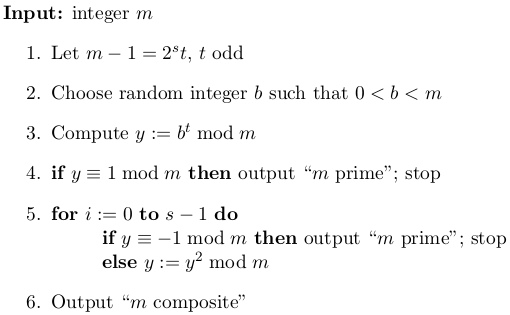
\includegraphics[width=11cm]{images/7-miller-rabin}
    \caption{The Miller-Rabin primality test}
  \end{centering}
\end{figure}

\subsubsection*{Correctness}
Even if the algorithm yields ``prime'' for $m$, we cannot be
completely sure if $m$ really is prime. On the other hand, if it
yields ``composite'', we know that it is \emph{not} a prime.

It can be shown that Miller-Rabin has at most $1/4$ probability of
yielding a false-positive. This can be countered by doing several
iterations with different random values for $b$. This lowers the
chance of the algorithm being wrong by $\frac{1}{4}^l$, where $l$ is
the number of different values for $b$ tested.
\clearpage

\section{The discrete logarithm problem modulo p and El-Gamal encryption}
%%% Local Variables:
%%% mode: latex
%%% TeX-master: "../index"
%%% End:

% Recommended:
% El-Gamal with formulas
% DLP and how El-Gamal uses it

\subsection{Agenda}
\begin{enumerate}
\item El-Gamal
\item DLP
\end{enumerate}

\subsection{Discrete log problem modulo a prime}
%%% Local Variables:
%%% mode: latex
%%% TeX-master: "../index"
%%% End:

Given a prime $p$ and $\alpha, \beta \in \mathbb{Z}_p^*$ find $a \in \mathbb{Z}_{p-1}$

\textbf{Problem:} For $\beta \equiv \alpha^a \mod p$, find $a$

\textbf{Example:} For $5^a \mod 17 = 4$, find $a$ given 5, 17 and 4. Solution is $a = 12$

\textbf{Requirements}
\begin{enumerate}
\item $p$ must be a large prime\\
  Since $a \in \mathbb{Z}_p$ one can just try all possible $a$s

\item $p - 1$ must have at least one large prime factor to make it
  difficult to prime factor

\item Smallest $m$ for which $\alpha^m \equiv 1 \mod p$ must be large,
  e.i. $\alpha$ should have a high order modulus $p$. \\
  If $\alpha^m
  \equiv 1 \mod p$ then $\alpha^m \equiv \alpha^{a \mod m} \mod p$ so
  there are only $m$ values to check.

  \textbf{Proof:} We can write $a = mq + r$ implying that $r = a \mod m$. Then
  \[ \alpha^a \equiv \alpha^{mq + r} \equiv \alpha^r\alpha^{mq} \equiv
  \alpha^r(\alpha^m)^q \equiv \alpha^r\cdot 1 \equiv \alpha^r \equiv
  \alpha^{a \mod m} \mod p\]
\end{enumerate}
\clearpage

\section{El-Gamal digital signatures}
%%% Local Variables:
%%% mode: latex
%%% TeX-master: "../index"
%%% End:

% Recommended:
% El-Gamal
% - Formulas (as much as possible)
% - In $\delta$, show that $k^{-1} \mod p-1$ has a multiplicative
%   inverse ($\gcd \equiv 1$), and then find it with Euclid's extended
%   algorithm.

\subsection*{Agenda}
\begin{enumerate}
\item DLP
\item El-Gamal
  \begin{itemize}
  \item Setup
  \item Properties of $k$
  \item Hash-functions
  \item Proof
  \end{itemize}
\end{enumerate}

\subsection{DLP}
%%% Local Variables:
%%% mode: latex
%%% TeX-master: "../index"
%%% End:

Given a prime $p$ and $\alpha, \beta \in \mathbb{Z}_p^*$ find $a \in \mathbb{Z}_{p-1}$

\textbf{Problem:} For $\beta \equiv \alpha^a \mod p$, find $a$

\textbf{Example:} For $5^a \mod 17 = 4$, find $a$ given 5, 17 and 4. Solution is $a = 12$

\textbf{Requirements}
\begin{enumerate}
\item $p$ must be a large prime\\
  Since $a \in \mathbb{Z}_p$ one can just try all possible $a$s

\item $p - 1$ must have at least one large prime factor to make it
  difficult to prime factor

\item Smallest $m$ for which $\alpha^m \equiv 1 \mod p$ must be large,
  e.i. $\alpha$ should have a high order modulus $p$. \\
  If $\alpha^m
  \equiv 1 \mod p$ then $\alpha^m \equiv \alpha^{a \mod m} \mod p$ so
  there are only $m$ values to check.

  \textbf{Proof:} We can write $a = mq + r$ implying that $r = a \mod m$. Then
  \[ \alpha^a \equiv \alpha^{mq + r} \equiv \alpha^r\alpha^{mq} \equiv
  \alpha^r(\alpha^m)^q \equiv \alpha^r\cdot 1 \equiv \alpha^r \equiv
  \alpha^{a \mod m} \mod p\]
\end{enumerate}

\subsection{El-Gamal Digital Signature}
%%% Local Variables:
%%% mode: latex
%%% TeX-master: "../index"
%%% End:

\subsubsection*{Setup}
\textbf{Public key:} $(p,\alpha,\beta)$ chosen such that DLP(p) is
difficult, and where:
\begin{itemize}
\item $p$ is an odd prime
\item $\alpha\in \mathbb{Z}_{p'}^*$
\item $\beta = \alpha^a \mod p$
\item $a \in \mathbb{Z}_{p-1} $
\end{itemize}

\textbf{Private key:} $a \in \mathbb{Z}_{p-1}$

\textbf{Signature:} for message $m \in \mathbb{Z}_{p-1}$
\begin{itemize}
\item Compute $x = H(m)$, where $H$ is a secure hashing function.
\item Choose a random $k \in \mathbb{Z}_{p-1}^*$.
\item $Sig(x) = (\gamma,\delta)$, where:
  \begin{align*}
    \gamma &= \alpha^k \mod p \\
    \delta &= (x-a\gamma)k^{-1} \mod p-1
  \end{align*}
\end{itemize}

\textbf{Verification:} for message $m \in \mathbb{Z}_{p-1}$ and
signature $(\gamma,\delta) \in \mathbb{Z}_p\times \mathbb{Z}_{p-1}$
\begin{itemize}
\item Compute $x = H(m)$, where $H$ is a secure hashing function.
\item $Ver(m, (\gamma,\delta))$ holds if:
  \[ \beta^{\gamma} \gamma^{\delta}= \alpha^x \mod p\]
\end{itemize}

\subsubsection*{Properties of k}
\begin{itemize}
\item Must be kept secret
\item Must have a multiplicative inverse $kx \equiv 1 \mod p - 1$.
  \begin{align*}
    \intertext{Must hold that}
    \gcd(p-1,k) &= 1
    \intertext{Can thereafter find multiplicative inverse Euclid's extended
      algorithm (\ref{sec:euclids-extended})}
    s \cdot (p-1) + t \cdot k &= 1
    \intertext{Where $t$ is the multiplicative inverse}
  \end{align*}
\end{itemize}

\subsubsection*{Hash-functions}
One can use any secure hash-function, as long as both parties agree on
using the same.

By hashing the message, one prevents forgery attacks. Without, an
active adversary could simply change the message and compute a new
signature.


\subsubsection*{Proof}
%%% Local Variables:
%%% mode: latex
%%% TeX-master: "../index"
%%% End:

We can ensure that El-Gamal will sign on $\alpha(x)$ due to the
following:

As $\beta$ is defined as $\beta = \alpha^{a}$ and from the signature, it's given:
\begin{align*}
  \gamma &= \alpha^k \mod p \\
  \delta &= (x - a \gamma)k^{-1} \mod p - 1 \\
\end{align*}

And from the verification it's given:
\[ \beta^{\gamma}\gamma^{\delta} \equiv \alpha^x \mod p\]

\begin{align*}
  \alpha^x &\equiv \beta^{\gamma}\gamma^{\delta} \mod p\\
  &\equiv \alpha^{a^{\gamma}} \gamma^{(x-a\gamma)k^{-1}} \mod p\\
  &\equiv \alpha^{a\gamma} \alpha^{k(x-a\gamma)k^{-1}} \mod p\\
  &\equiv \alpha^{a\gamma} \alpha^{x-a\gamma} \mod p\\
  &\equiv \alpha^{a\gamma} \alpha^{x}\alpha^{-a\gamma} \mod p\\
  &\equiv \alpha^x \mod p
\end{align*}

Because of Fermat's little theorem (\ref{sec:fermats-little}) the
following is possible: if $\alpha\in \mathbb{Z}_{p'}^*$:
\begin{align*}
  \alpha^{p-1} &\equiv 1 \mod p\\
  \alpha^p &\equiv \alpha \mod p\\
  \text{then}&\\
  \alpha^x \mod p &\equiv \alpha^{x \mod p-1} \mod p
\end{align*}


\clearpage

\section{Iterated hash functions, birthday paradox}
%%% Local Variables:
%%% mode: latex
%%% TeX-master: "../index"
%%% End:

% Recommended:
% Complexity of collisions (preimage)
% - Birthday paradox
% How to build hash functions
% - Blocks with padding
% - Merkle-Damgaard
% - Why is it secure?

\subsection*{Agenda}
\begin{enumerate}
\item Properties of hash-functions
\item Complexity of collisions
\item Iterated Hash-functions
\item Merkle-Damgård construction
\end{enumerate}

\subsection{Properties of Hash functions}
\textbf{Hash functions} takes a input of a binary string of arbitrary
length and returns a binary string of fixed length.
\begin{figure}[H]
  \centering
  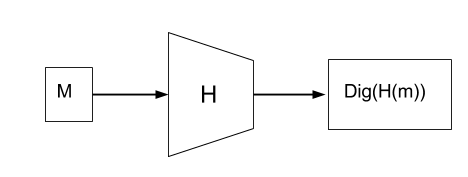
\includegraphics[scale=0.4]{images/10-hash}
  \caption{Model for hashing a message}
\end{figure}

\textbf{The ideal Hash function} has 4 main properties:
\begin{itemize}
\item It is easy to compute the hash value for any given message
\item It is infeasible to generate a message that has a given hash (pre-image)
\item It is infeasible to modify a message without changing the hash
\item It is infeasible to find two different messages with the same hash (collision)
\end{itemize}

\subsection{Complexity of collisions}

\begin{align*}
&\mbox{\textbf{Attack}}\hspace{2cm}&\mbox{\textbf{Rough Complexity}}\\
&\mbox{Collision}\hspace{2cm}&\sqrt{2^n}=2^{n/2}\\
&\mbox{2nd preimage}\hspace{2cm}&2^n\\
&\mbox{Preimage}\hspace{2cm}&2^n\\
\end{align*}
\subsubsection*{Finding complexity of collision attack}
Probability of finding a collision is found with the birthday paradox. Given a function $f$ that maps
values to $q$ different outputs, the probability of finding a
collision after $n$ randomly selected inputs is

\[ p(n; q) \approx 1 - e^{\frac{-n(n-1)}{2\cdot q}}\]

This expression can be inverted to $n(p; q)$ describing how many tries
$n$ it takes to reach a probability $p$ of collision

\[ n(p; q) \approx \sqrt{2q \ln \frac{1}{1 - p}} \]

To achieve $50\%$ chance of collision

\[ n(0.5; q) = 1.1774 \sqrt{q} \]

\textbf{Example:} For a 128 bit hash there are $2^{128}$ different
hashes, and the number of tries needed to achieve $50\%$ chance of
collision is then

\[ 1.1774 \sqrt{2^{128}} \approx 2.17 \cdot 10^{19} \]

\subsection{Iterated Hash-functions}
\begin{itemize}
\item Hash-function must be able to process an arbitrary-length
  message into a fixed-length output.
\item Can be achieved by breaking the input up into a series of
  equal-sized blocks, and operating on them in sequence using a
  one-way compression function
\item To make sure the message fits the blocks of the compression
  function, we apply a padding function.
\item We will show that this provides a method for showing that if one
  finds a collision for the hashing function, one also found a
  collision for the compression function.
\end{itemize}

\begin{figure}[H]
  \begin{centering}
    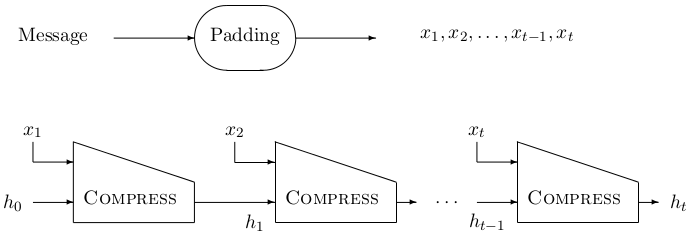
\includegraphics[width=12cm]{images/10-it-hash}
    \caption{Model of iterated hash-functions}
  \end{centering}
\end{figure}

% \begin{figure}[H]
%   \centering
%   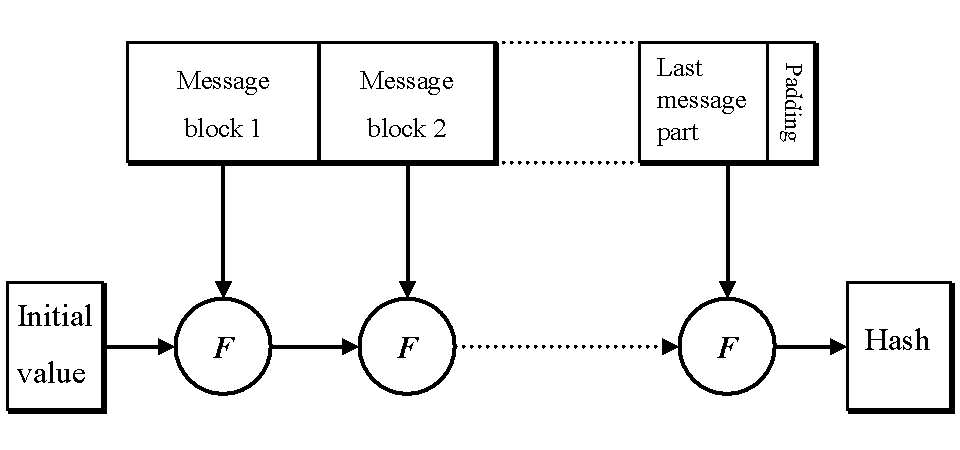
\includegraphics[scale=0.3]{images/10-padding}
%   \caption{Model for hashing using padding}
% \end{figure}

\subsection{The Merkle-Damgård Construction}
Let $h$ be a compression function:
\[ h: \{0,1\}^N \rightarrow \{0,1\}^n \quad \text{where } N > n \]

We construct a hash-function $H$, for some large value $M$:
\[ H: \{0,1\}^M \rightarrow \{0,1\}^n \]

Typical values of $M$ can be $2^{64}-1$ or $2^{128}-1$.

\subsubsection*{Padding}
Begin by computing $l_M$ such that it is the smallest possible where
it holds that $2^{l_M} -1 \ge M$.
\begin{itemize}
\item Let $x \in \{0,1\}^v$ be a $v$-bit string to be hashed
\item First append a one-bit to $x$, that is, $x := x | ‘1’$. Now the length of $x$ is $v + 1$.
\item Let $s$ be the least positive integer such that $v + 1 + s +
  l_M$ is a multiple of $N - n$,\\ e.i. $s \equiv - (v + 1 + l_M) \mod
  (N-n)$
\item Append $s$ zero-bits to $x$.
\item Append to $x$ a block of $l-M$ bits which contains the binary representation of the integer
\end{itemize}

\subsubsection*{Collision}
A hash function built with the Merkle–Damgård construction is as
resistant to collisions as is its compression function; any collision
for the full hash function can be traced back to a collision in the
compression function.

\textbf{Proof}\\
Let $IV \in {0, 1}^n$ be a fixed, randomly chosen value. Let $h$ and $H$ be as above.

Assume there is a collision for $H$. We want to show that then there
is also a collision for $h$ somewhere. Thus, we have two distinct
strings $x \not= x'$, such that $H(x) = H(x')$.

Let $z$ and $z'$ be
the results of padding $x$ and $x'$ according to above rule. Then $z =
z'$.
\begin{align*}
  z = (z_1 , z_2 , \ldots , z_t) \\
  z' = (z'_1 , z'_2 , \ldots , z'_s )
\end{align*}
We will assume that the message lengths that are appended in the
padding rule are (fully) contained in the last blocks, $z_t$ and
$z'_s$.

\textbf{Assume first that $t = s$} \\
We therefore have
\[ H(x) = H(x') \Rightarrow h(h_{t-1} , z_t) = h(h'_{s-1} , z'_s) \]
which gives a collision for $h$, since $z_t$ contains a binary representation
of $t$ and $z'_s$ contains a binary representation of $s$ and $t = s$.

\textbf{Assume next that $t = s$} \\
We now have
\[ H(x) = H(x') \Rightarrow h(h_{t-1} , z_t) = h(h'_{t-1}, z'_t) \]
which gives a collision for $h$, or it holds that
\[ (h_{t-1} , z_t) = (h'_{t-1} , z'_t) \]
In the latter case, this means that
\[ h_{t-1} = h'_{t-1} \Rightarrow h(h_{t-2} , z_{t-1}) = h(h'_{t-2} , z'_{t-1}) \]
Thus, either there is a collision for $h$, or it holds that
\[ (h_{t-2} , z_{t-1}) = (h'_{t-2} , z'_{t-1}) \]

Continuing in this fashion, one finds either a collision for $h$ or it
holds that
\[ z_{t-i} = z_{t-i}\ , \quad  i = 0 \ldots t-1 \]

The latter cannot be true since it was assumed that $z = z'$.

\clearpage

\section{The discrete logarithm problem modulo p and Diffie-Hellman key agreement}
%%% Local Variables:
%%% mode: latex
%%% TeX-master: "../index"
%%% End:

\subsection{Recommended}
\begin{itemize}
\item DLP
\item Problem with Man-in-the-Middle
\item How to fix it
\end{itemize}

\clearpage

\section{Secret Sharing}
%%% Local Variables:
%%% mode: latex
%%% TeX-master: "../index"
%%% End:

% Recommended:
% $(t, w)$
% - Why can $t$-people reconstruct the key?
% - Why cannot less than $t$-people reconstruct the key?

\subsection*{Agenda}
\begin{enumerate}
\item Purpose
\item Shamir's threshold scheme
\item Further discussion
\end{enumerate}

\subsection{Purpose}
What if you could give  only shares of the secret key to your
friends, but only need a subset of the shares to reconstruct the
secret key? Now none of your friends can alone decrypt you data, and
it doesn't matter if a friend or two loses their share. This is
\emph{secret sharing}.

\subsection{Shamir's threshold scheme}
\subsubsection*{Setup}
\begin{itemize}
\item $(t, w)$, where $t$ is the threshold and $w$ is the number of shareholders
\item Participants: Keyholder $H$, shareholders $S_1, \ldots, S_w$
\item Secret key: $k$
\item $H$ chooses:
  \begin{itemize}
  \item a prime $p$, such that $p \ge w + 1$
  \item a random polynomial over a final field of size $p$
    \[ f(x) = k + \sum\limits_{j=1}^{t-1} c_jx^j \mod p \]
    of degree $t-1$, where $c_j$s are chosen at random
  \end{itemize}
\item $H$ computes $(x_i, f(x_i))$ for $i  = 1, \ldots, w$
\end{itemize}

\subsubsection*{Re-construction}
\begin{figure}[H]
  \begin{equation}\label{eq:lagrange}
    f(x) = \sum\limits_{i=1}^t y_1 \prod\limits_{j=1, j\not=i}^t \frac{x-x_j}{x_i-x_j}
  \end{equation}
  \caption{Lagrange Interpolation Formula}
\end{figure}

\begin{itemize}
\item Input: $t$ shares $(x_i, y_i)$ for $i = 1, \ldots, t$
\item $H$ re-constructs the secret key $k$ by using Lagrange Interpolation Formula (\ref{eq:lagrange})
  \[ k = f(0) = \sum\limits_{i=1}^t y_i \prod\limits_{j=1, j\not=i}^t \frac{x_j}{x_j-x_i} \]
\end{itemize}

In this scheme, any $t$ out of $w$ shares may be used to recover the
secret. The system relies on the idea that you can fit a unique
polynomial of degree $t-1$ to any set of $t$ points that lie on the
polynomial. It takes two points to define a straight line, three
points to define a parabola, four points to define a cubic
curve, and so on. That is it takes $t$ points to define a polynomial
of degree $t-1$.

\subsection{Further discussion}
\textbf{$t$ shareholders} \\
There is only one polynomial $f(x)$ over $\mathbb{Z}_p$ of degree at
most $t-1$, such that $f(x_i) = y_i$ for $i = 1,\ \dots,\
t$. Therefore, $t$ shareholders with the shares $\{(x_1,y_1),\
(x_2,y_2),\ \ldots,\ (x_t,y_t)\}$, can re-construct the polynomial
$f(x)$ using the Lagrange Interpolation Formula~(\ref{eq:lagrange}) and
compute the secret key for $f(0)$.

Further, if we describe the shares as follows
\begin{equation}
  \begin{pmatrix}
    1      & x_1    & x_1^2    & \cdots & x_1^{t-1} \\
    1      & x_2    & x_2^2    & \cdots & x_2^{t-1} \\
    \cdots & \cdots & \cdots  & \cdots & \cdots \\
    1      & x_{t-1} & x_{t-1}^2 & \cdots & x_{t-1}^{t-1} \\
    1      & x_t    & x_t^2    & \cdots & x_t^{t-1}
  \end{pmatrix}
  \begin{pmatrix}
    c_0 \\
    c_1 \\
    c_2 \\
    \cdots \\
    c_{t-1}
  \end{pmatrix} =
  \begin{pmatrix}
    y_0 \\
    y_1 \\
    y_2 \\
    \cdots \\
    y_t
  \end{pmatrix} \mod p
\end{equation}

Since $p$ is assumed to be a prime, and since $x_i \not= x_j$ for $1 \le i
< j \le t$, Theorem 2.4.3 tells us that the determinant of the matrix
is nonzero. As we also know that any nonzero element modulo $p$ (a
prime) has a multiplicative inverse, so the matrix above can be
inverted. Thus, re-constructing the polynomial $f(x)$.
\\

\textbf{$t-1$ shareholders} \\
If $t-1$ shareholders pool their shares, denoted $\{(x_1,y_1),\
(x_2,y_2),\ \ldots,\ (x_{t-1},y_{t-1})\}$, and determine that $f(0) = k'$.

\begin{equation}
  \begin{pmatrix}
    1      & x_1    & x_1^2    & \cdots & x_1^{t-1} \\
    1      & x_2    & x_2^2    & \cdots & x_2^{t-1} \\
    \cdots & \cdots & \cdots  & \cdots & \cdots \\
    1      & x_{t-1} & x_{t-1}^2 & \cdots & x_{t-1}^{t-1} \\
    1      & 0      & 0       & \cdots & 0
  \end{pmatrix}
  \begin{pmatrix}
    c_0 \\
    c_1 \\
    c_2 \\
    \cdots \\
    c_{t-1}
  \end{pmatrix} =
  \begin{pmatrix}
    y_0 \\
    y_1 \\
    y_2 \\
    \cdots \\
    k'
  \end{pmatrix} \mod p
\end{equation}

As for the same argument as above, for any value of $k'$ we can
re-construct an unique polynomial that could have generated their
shares, for which $f(0) = k'$. Hence, the shareholders have no
information about the value of the secret key.

\end{document}
